\documentclass[10pt, twoside]{article}
\title{The area between functions $x^{\frac{1}{n}}$ and $x^n$ in the domain $0 \le x \le 1$ is equal to $\frac{x-1}{x+1}$}
\author{Amit Kumar}
\date{\today}
\usepackage[a4paper, margin=0.75in]{geometry}
\usepackage[page]{appendix}
\usepackage{amsmath}
\usepackage{amssymb}
\usepackage{mathtools}
\usepackage{pythonhighlight}
\usepackage{graphicx}
\usepackage{float}
\usepackage{url}
\begin{document}
\maketitle
\section{Abstract}
When the graphs of functions $y=x^{\frac{1}{n}}$ and $y=x^n$ are plotted [in the domain $0 \le x \le 1$,range/co-domain $0 \le y \le 1$] then an area is carved between the two functions by the virtue of intersection of the two graphs (at 0 and 1). If we consider the area formed by the unit square [$0 \le x \le 1$ and $0 \le y \le 1$] to be 100\%, then the above mentioned `carved out area due to intersection' is a function of `$n$' and grows as the value of `$n$' grows, asymptotically reaching 100\% for n=$\infty$. The relationship between the 'carved area' and `$n$' is simply: $\Delta = (\frac{x-1}{x+1}\times{100})\%$ of the total area between the unit square formed.
\section{Derivation}
Let us see three plots to understand the behavior of the area carved out by the intersection of two curves. Below are the curves for n=2, 3 and 10 (Figure \ref{Area_2_3_10}). 
\begin{figure}[h!]
\includegraphics[width=\linewidth]{All_Three_Plots.png}
\caption{The area made by intersection is an increasing function of n}
\label{Area_2_3_10}
\end{figure}
It is easy to calculate the area formed by the intersection between the two functions by going through these 3 steps.
\begin{enumerate}
\item Calculate the area under the function $x^{\frac{1}{n}}$.
\item Calculate the area under the function $y=x^n$.
\item Subtract the second step from the first step.
\end{enumerate}
Thus we can calculate the area as below.
\begin{align*}
 \Delta &= \int_{0}^{1}x^{\frac{1}{n}}dx - \int_{0}^{1}x^{n}dx \\
 &= \frac{x^{\frac{1}{n}+1}}{\frac{1}{n}+1} \Big|_0^1 - \frac{x^{n+1}}{n+1} \Big|_0^1 \\
 &= \Big[\frac{1^{\frac{1}{n}+1}}{\frac{1}{n}+1} - \frac{0^{\frac{1}{n}+1}}{\frac{1}{n}+1}\Big] - \Big[\frac{1^{n+1}}{n+1} - \frac{0^{n+1}}{n+1} \Big] \\
 &= \frac{1}{\frac{1}{n}+1} - \frac{1}{n+1}\\
 &= \frac{n}{n+1} - \frac{1}{n+1} \\
 &= \frac{n-1}{n+1}
\end{align*}
For $n=1$ there should be no area while for $n=\infty$ the area should cover the whole square intuitively. As a sanity check we can calculate the area for $n=1$ and $n=\infty$ and we find the results to be $0$ and $1$ respectively, as expected. 

\section{Discussion}
Below is a table for different values of n (from 1 to 100).\newline
\begin{tabular}{|l || l |}
	\hline
	\textbf{n} & \textbf{fraction} \\
	\hline
	1 & 0.0000 \\
	\hline
	2 & 0.3333 \\
	\hline
	3 & 0.5000 \\
	\hline
	4 & 0.6000 \\
	\hline
	5 & 0.6667 \\
	\hline
	6 & 0.7143 \\
	\hline
	10 & 0.8182 \\
	\hline
	25 & 0.9231 \\
	\hline
	50 & 0.9608 \\
	\hline
	100 & 0.9802 \\
	\hline
\end{tabular}
\newline
\newline
This observation can be turned into a plot as below (Figure \ref{n_vs_frac}).\newline
\begin{figure}[h!]
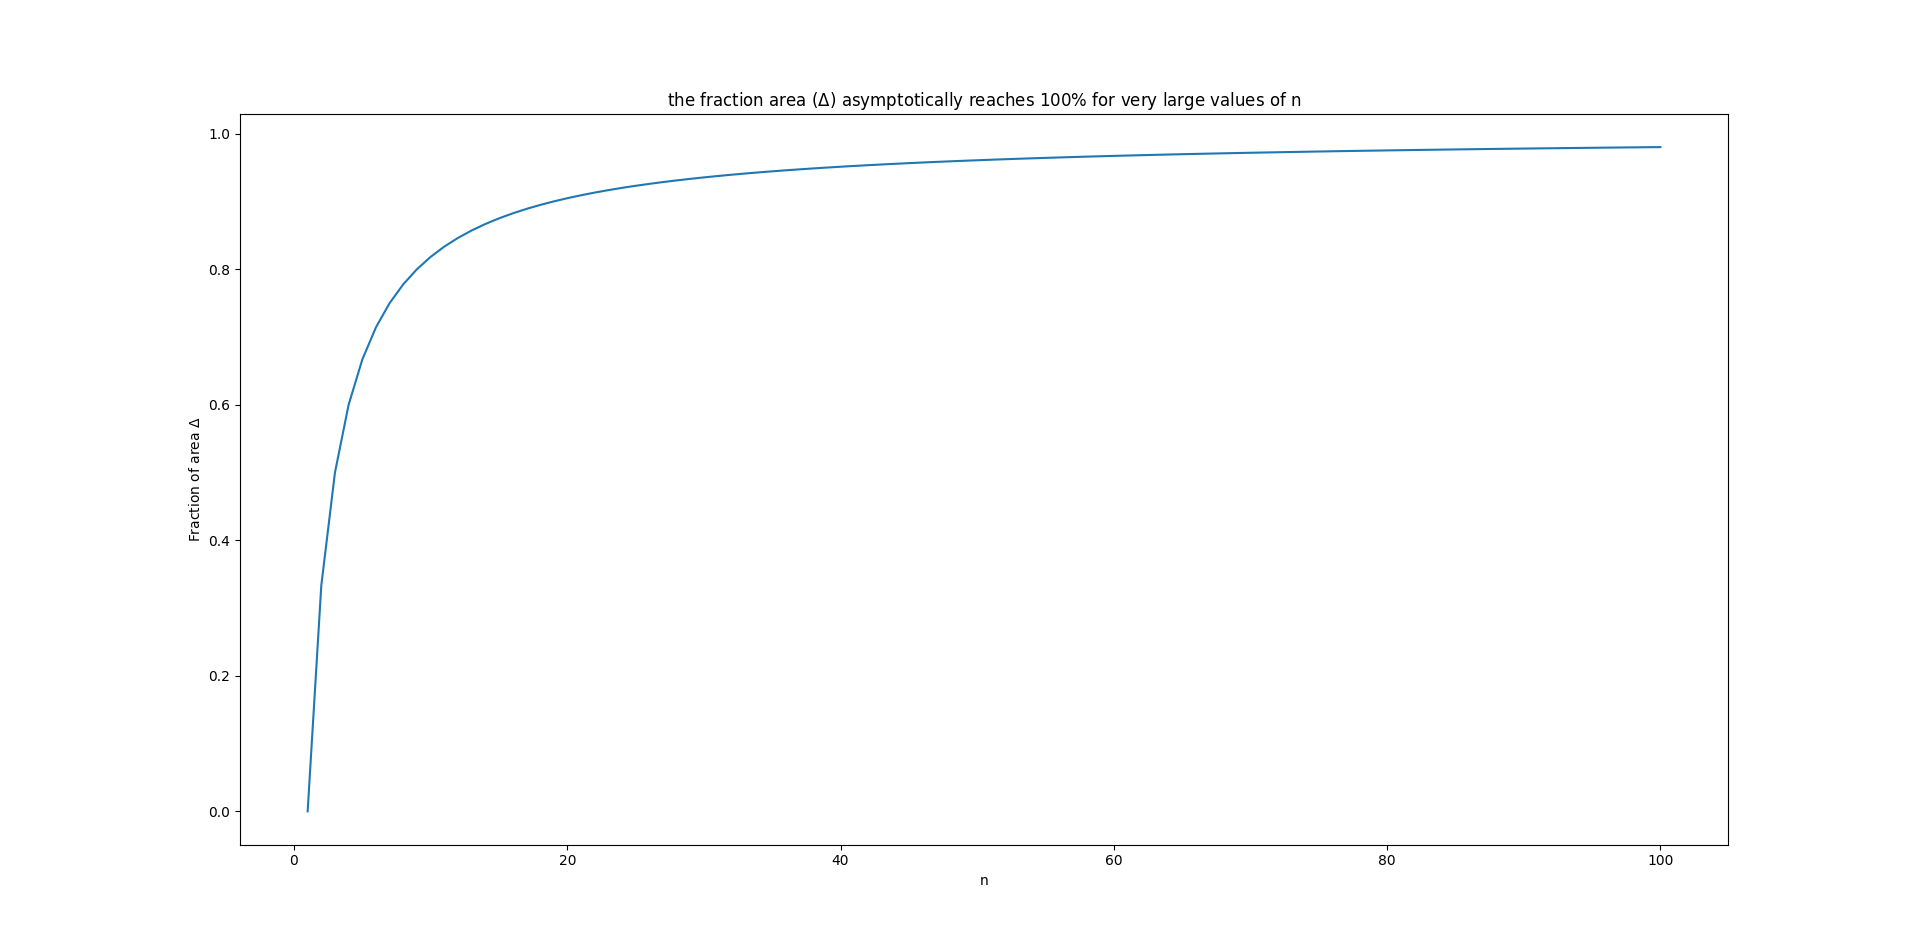
\includegraphics[width=\linewidth]{Overall_Plot.png}
\caption{The fraction asymptotically reaches 100\% for large values of n}
\label{n_vs_frac}
\end{figure}
\newline
As we can see this equation is a special case of  Möbius-Transformation. A Möbius-Transformation transformation is defined as $f(z) = \frac{az+b}{cz+d}$, where $ad-bc \ne 0$. In this context this function is special since $z$ is replaced by $x$ and $a=c=d=1 \ne b=-1$. Please see \url{https://math.stackexchange.com/questions/5059632/does-the-function-y-fracx-1x1-have-a-name} for some very helpful comments on this. 
\end{document}